
\documentclass[10 pt,usenames,dvipsnames, oneside]{article}
\usepackage{../../modelo-fracoes}
\graphicspath{{../../../Figuras/licao03/}}


\begin{document}

\begin{center}
  \begin{minipage}[l]{3cm}

\includegraphics[width=2cm]{../../../Figuras/logo}       
\end{minipage}\hfill
\begin{minipage}[r]{.8\textwidth}
 {\Large \scshape Atividade: Quantidades na reta (formas)}  
\end{minipage}
\end{center}
\vspace{.2cm}

\ifdefined\prof
%Caixa do Para o Professor
\begin{goals}
%Objetivos específicos
\begin{enumerate}
\item Representar frações na reta numérica.
\item Associar, na reta numérica e a partir de modelos contínuos, a unidade ao número 1.
\end{enumerate}

\tcblower

%Orientações e sugestões
\begin{itemize}
\item Esta atividade propõe, a partir de modelos contínuos, a associação de quantidades a pontos da reta numérica. Para isso, em cada item estão destacados na reta, além do 0 e do 1, frações e marcações apropriadas às subdivisões correspondentes. Por exemplo, para o quadrado que  está dividido em nonos, o segmento unitário traz uma marcação que destaca a subdivisão em nove partes iguais e destaca as frações $\frac{4}{9}$ e $\frac{5}{9}$.
\item Para responder, o aluno pode simplesmente ligar com uma linha a representação em imagem ao ponto da reta correspondente à fracão identificada.
\item Observe que o enunciado não determina a unidade. É provável que o aluno escolha as regiões totalmente coloridas em vermelho como unidade. A solução considera esse caso. No entanto, a região colorida em vermelho de qualquer uma das figuras pode ser considerada unidade. Essa escolha torna a solução mais complexa nos itens c) e f). Por exemplo, no item c), se a região em vermelho da Figura A for a unidade, a Figura B, todo o quadrado em vermelho, corresponderia a $\frac{9}{5}$. Fique atento às respostas dos seus alunos e avalie explorar essa discussão em sala.
\end{itemize}
\end{goals}

\bigskip
\begin{center}
{\large \scshape Atividade}
\end{center}
\fi

  Que fração da figura está pintada de vermelho? Ligue cada figura ao número correspondente  destacado na reta numérica.
  
\begin{longtable}{lccc}
%retangulos
a)& Figura A & & Figura B\\
& \begin{tikzpicture}[x=30mm,y=30mm,scale=.6]
  \draw[ fill=attention] (-1.8,0) rectangle (0,1.2);
 % \node [above] at (-.9,1.2) {Figura 1};
\end{tikzpicture}
&&

\begin{tikzpicture}[x=30mm,y=30mm,scale=.6]
\draw[fill=common, fill opacity=.3] (0,0) rectangle (1.8,1.2);
%\node [above] at (.9,1.2) {Figura 2};
\draw[fill=attention] (0,0) -- (0,1.2) --(1.8,0)--cycle;
\end{tikzpicture}

\\

\multicolumn{4}{c}{
\parbox[c][.7cm][t]{8cm}{ } }

\\

&\multicolumn{3}{c}{
\begin{tikzpicture}[x=45mm,y=45mm]
\draw[->] (-0.5,0) -- (1.5,0) ; %edit here for the axis
\foreach \x in  {0,1} % edit here for the vertical lines
\draw[shift={(\x,0)},color=black] (0,3pt) -- (0pt,-3pt)
node[below] {$\x$};
\draw[shift={(0.5,0)},color=black] (0,3pt) -- (0pt,-3pt)
node[below] {$\frac{1}{2}$};
\end{tikzpicture}
}

\\\ifdefined\prof\clearpage\fi
% item b)
b)& Figura A & & Figura B \\
 %triangulos
& \begin{tikzpicture}[x=30mm,y=30mm]
\def\scale{.6}% to rescale the polygons only.

\foreach \x in {90,210,330}{
\draw[attention,fill=attention, shift={(0,0.6)}, scale=\scale] (\x:0.7) -- (\x + 120: 0.7) -- (0,0)--cycle;
\draw[shift={(0,0.6)}, scale=\scale] (\x:0.7) -- (\x + 120: 0.7);}
\draw[shift={(0,0.6)}, scale=\scale] (-90:0.35) -- (30: 0.35) -- (150: 0.35) -- cycle;
 %\node [above] at (-.9,1.2) {Figura 1};
\end{tikzpicture}
&&
\begin{tikzpicture}[x=30mm,y=30mm]
\def\scale{.6}% to rescale the polygons only.
\fill[shift={(1,0.6)}, scale=\scale, common, fill opacity=.3] (90:0.7) -- (210: 0.7)--(330:.7)--cycle;
\foreach \x in {90,210,330}{
\draw[shift={(1,0.6)}, scale=\scale] (\x:0.7) -- (\x + 120: 0.7);}
\draw[fill=attention, shift={(1,0.6)}, scale=\scale] (-90:0.35) -- (30: 0.35) -- (150: 0.35) -- cycle;
% \node [above] at (.9,1.2) {Figura 2};
\end{tikzpicture}

\\

\multicolumn{4}{c}{
\parbox[c][.7cm][t]{8cm}{ } }

\\
&\multicolumn{3}{c}{
\begin{tikzpicture}[x=60mm,y=60mm]
\draw[->] (-1/4,0) -- (1+1/4,0) ; %edit here for the axis
\foreach \x in  {0,0.25,...,1}{ % edit here for the vertical lines
\draw[shift={(\x,0)},color=black] (0,3pt) -- (0pt,-3pt);}
\foreach \x in  {0,1}
\draw[shift={(\x,0)},color=black] (0,3pt) -- (0pt,-3pt) node[below] {$\x$};
\foreach \x in  {1,3}
\draw[shift={(\x/4,0)},color=black] (0,3pt) -- (0pt,-3pt) node[below] {$\frac{\x}{4}$};
\end{tikzpicture}}
\\

c) & Figura A & & Figura B \\

%quadrados


& \begin{tikzpicture}[x=30mm,y=30mm]
\def\scale{.6}
%
\draw[fill=common, fill opacity=.3, scale=\scale] (-1.2,0) rectangle (0,1.2);
\draw[fill=attention, scale=\scale] (-1.2,0) rectangle (-0.8,.4);
\draw[fill=attention, scale=\scale] (-.4,0) rectangle (0,.4);
\draw[fill=attention, scale=\scale] (-1.2,0.8) rectangle (-0.8,1.2);
\draw[fill=attention, scale=\scale] (-.4,0.8) rectangle (0,1.2);
\draw[fill=attention, scale=\scale] (-.8,0.4) rectangle (-0.4,.8);

% \draw[ fill=attention, scale=\scale] (-1.2,.8) rectangle (0,1.2);

% \draw[fill=common, fill opacity=.3, scale=\scale] (-0.8,0) rectangle (-.4,.4);
% \draw[ fill=attention, scale=\scale] (-0.8,.4) rectangle (-0.4,.8);
% \draw[fill=common, fill opacity=.3, scale=\scale] (-0.8,.8) rectangle (-.4,1.2);
\end{tikzpicture}
&&
 \begin{tikzpicture}[x=30mm,y=30mm]
\def\scale{.6}
\draw[fill=attention, scale=\scale] (0,0) rectangle (1.2,1.2);
\end{tikzpicture}

\\

\multicolumn{4}{c}{
\parbox[c][.7cm][t]{8cm}{ } }

\\

&\multicolumn{3}{c}{
\begin{tikzpicture}[x=45mm,y=45mm]
\draw[->] (-0.5,0) -- (1.5,0) ; %edit here for the axis
\foreach \x in  {0,0.1111,...,1}{ % edit here for the vertical lines
\draw[shift={(\x,0)},color=black] (0,3pt) -- (0pt,-3pt);}
\foreach \x in  {0,1}
\draw[shift={(\x,0)},color=black] (0,3pt) -- (0pt,-3pt) node[below] {$\x$};
\foreach \x in  {4,5}
\draw[shift={(\x/9,0)},color=black] (0,3pt) -- (0pt,-3pt) node[below] {$\frac{\x}{9}$};
\end{tikzpicture}}
\\

%hexagonos
d) & Figura A & & Figura B \\

& \begin{tikzpicture}[x=30mm,y=30mm]
\def\scale{.6}% to rescale the polygons only.

%hexagon on the left
\fill[shift={(0,0.6)}, fill=attention, scale=\scale] (0,0) -- (90:0.7) -- (150:0.7)-- (210:.7);
\fill[shift={(0,0.6)}, fill=common, fill opacity=.3, scale=\scale] (0,0) -- (90:0.7) -- (30:0.7)-- (-30:.7) -- (-90:.7) -- (-150:.7)--cycle;
\foreach \x in {30,90,...,330}{
\draw[shift={(0,0.6)}, scale=\scale] (\x:0.7) -- (\x + 60: 0.7);
\draw[shift={(0,0.6)}, scale=\scale] (0,0) -- (\x:0.7);}
\end{tikzpicture}
&&
\begin{tikzpicture}[x=30mm,y=30mm]
\def\scale{.6}% to rescale the polygons only.

%hexagon on the right
\foreach \x in {30,90,...,330}{
\draw[shift={(1,0.6)}, fill=attention,attention, scale=\scale] (\x:0.7) -- (\x + 60: 0.7) --(0,0) --cycle;
\draw[shift={(1,0.6)}, fill=attention, scale=\scale] (\x:0.7) -- (\x + 60: 0.7);}
\end{tikzpicture}

\\

\multicolumn{4}{c}{
\parbox[c][.7cm][t]{8cm}{ } }

\\
&\multicolumn{3}{c}{
\begin{tikzpicture}[x=68mm,y=68mm]
\draw[->] (-1/6,0) -- (1+1/6,0) ; %edit here for the axis
\foreach \x in  {0,0.1667,...,1}{ % edit here for the vertical lines
\draw[shift={(\x,0)},color=black] (0,3pt) -- (0pt,-3pt);}
\foreach \x in  {0,1}
\draw[shift={(\x,0)},color=black] (0,3pt) -- (0pt,-3pt) node[below] {$\x$};
\foreach \x in  {1,2}
\draw[shift={(\x/3,0)},color=black] (0,3pt) -- (0pt,-3pt) node[below] {$\frac{\x}{3}$};
\end{tikzpicture} }
\\
\ifdefined\prof
\else
\clearpage
\fi
e) & Figura A & Figura B & Figura C \\

%os baianos e os novos retangulos
& \begin{tikzpicture} [x=30mm,y=30mm]
\def\scalefig {.6}
\draw[shift={(-.35*\scalefig,0.3)}, fill=attention, scale=\scalefig] (-1.5,0) rectangle (-0.5,1.2);
\draw[shift={(-.35*\scalefig,0.3)}, scale=\scalefig, fill=common, fill opacity=.3] (-.5,0) rectangle (0,1.2);
\draw[shift={(-.35*\scalefig,0.3)}, scale=\scalefig] (-1,0) -- (-1,1.2);
\end{tikzpicture}
&
\begin{tikzpicture} [x=30mm,y=30mm]
\def\scalefig {.6}
\draw[shift={(1.25*\scalefig,0.3)}, fill=common, fill opacity=.3, scale=\scalefig] (-1.5,0) rectangle (-1,1.2);
\draw[shift={(1.25*\scalefig,0.3)}, scale=\scalefig, fill=common, fill opacity=.3] (-1,0) rectangle (0,1.2);
\draw[shift={(1.25*\scalefig,0.3)}, scale=\scalefig] (-.5,0) -- (-.5,1.2);
\end{tikzpicture}
&
\begin{tikzpicture} [x=30mm,y=30mm]
\def\scalefig {.6}
\draw[shift={(1.35*\scalefig,0.3)}, fill=attention, scale=\scalefig] (0,0) rectangle (1.5,1.2);
\draw[shift={(1.35*\scalefig,0.3)}, scale=\scalefig] (.5,0) -- (.5,1.2);
\draw[shift={(1.35*\scalefig,0.3)}, scale=\scalefig] (1,0) -- (1,1.2);
\end{tikzpicture}

\\

\multicolumn{4}{c}{
\parbox[c][.7cm][t]{8cm}{ } }

\\
&\multicolumn{3}{c}{
\begin{tikzpicture}[x=55mm,y=55mm]
 \begin{scope}[shift={(-.3,0)}]
\draw[->] (-1/3,0) -- (1.33,0) ; %edit here for the axis
\foreach \x in  {0,1} % edit here for the vertical lines
\draw[shift={(\x,0)},color=black] (0,3pt) -- (0pt,-3pt)
node[below] {$\x$};
\foreach \x in {1,2}
\draw[shift={(\x/3,0)},color=black] (0,3pt) -- (0pt,-3pt)
node[below] {$\frac{\x}{3}$};
\end{scope}
\end{tikzpicture}}
\\

f) & Figura A & Figura B & Figura C \\

&\begin{tikzpicture}[scale=.48]
\fill[common, fill opacity=.3] (0,0) rectangle (45,45);
 \fill[attention] (0,33.75) rectangle (33.75,45);
 \draw[step=11.25, fill=attention] (0,0) grid (45,45);
\end{tikzpicture}
&
\begin{tikzpicture}[scale=.48]
\draw[fill=attention] (0,0) rectangle (45,45);
\end{tikzpicture}
&
\begin{tikzpicture}[scale=.48]
  \draw[fill=common, opacity=.3] (0,0) rectangle (45,45);
%  \draw[step=11.25, fill=white] (0,0) rectangle (45,11.25);
  \draw[fill=attention] (0,0) rectangle (33.75,33.75);
  \draw[step=11.25] (0,0) grid (45,45);
\end{tikzpicture}

\\

\multicolumn{4}{c}{
\parbox[c][.7cm][t]{8cm}{ } }



\\
&\multicolumn{3}{c}{
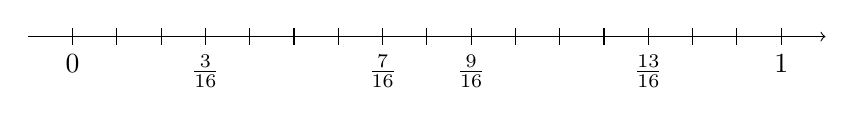
\begin{tikzpicture}[x=90mm,y=90mm]
 \draw[->] (-1/16,0) -- (1+1/16,0) ; %edit here for the axis
 \foreach \x in  {0,0.0625,...,1}{ % edit here for the vertical lines
 \draw[shift={(\x,0)},color=black] (0,3pt) -- (0pt,-3pt);}
\foreach \x in  {0,1}
\draw[shift={(\x,0)},color=black] (0,3pt) -- (0pt,-3pt) node[below] {$\x$};
\foreach \x in  {3,7,9,13}
\draw[shift={(\x/16,0)},color=black] (0,3pt) -- (0pt,-3pt) node[below] {$\frac{\x}{16}$};
\end{tikzpicture}
}
\end{longtable}

\ifdefined\prof
\clearpage
\begin{solucao}

\begin{enumerate}
\item \adjustbox{valign=t}
{
\begin{tikzpicture}[x=30mm,y=30mm]
\draw[->] (-0.5,0) -- (1.5,0) ; %edit here for the axis
\foreach \x in  {0,1} % edit here for the vertical lines
\draw[shift={(\x,0)},color=black] (0,3pt) -- (0pt,-3pt)
node[below] {$\x$};
\draw[shift={(0.5,0)},color=black] (0,3pt) -- (0pt,-3pt)
node[below] {$\frac{1}{2}$};

\fill[common] (.5,0) circle (3pt) node[above, black] {Fig. B};
\fill[common] (1,0) circle (3pt) node[above, black] {Fig. A};
\end{tikzpicture}
}


\item \adjustbox{valign=t}
{
\begin{tikzpicture}[x=40mm,y=40mm]
\draw[->] (-1/4,0) -- (1+1/4,0) ; %edit here for the axis
\foreach \x in  {0,0.25,...,1}{ % edit here for the vertical lines
\draw[shift={(\x,0)},color=black] (0,3pt) -- (0pt,-3pt);}
\foreach \x in  {0,1}
\draw[shift={(\x,0)},color=black] (0,3pt) -- (0pt,-3pt) node[below] {$\x$};
\foreach \x in  {1,3}
\draw[shift={(\x/4,0)},color=black] (0,3pt) -- (0pt,-3pt) node[below] {$\frac{\x}{4}$};

\fill[common] (1/4,0) circle (3pt) node[above, black] {Fig. B};
\fill[common] (1,0) circle (3pt) node[above, black] {Fig. A};

\end{tikzpicture}
}

\item \adjustbox{valign=t}
{
\begin{tikzpicture}[x=30mm,y=30mm]
\draw[->] (-0.5,0) -- (1.5,0) ; %edit here for the axis
\foreach \x in  {0,0.1111,...,1}{ % edit here for the vertical lines
\draw[shift={(\x,0)},color=black] (0,3pt) -- (0pt,-3pt);}
\foreach \x in  {0,1}
\draw[shift={(\x,0)},color=black] (0,3pt) -- (0pt,-3pt) node[below] {$\x$};
\foreach \x in  {4,5}
\draw[shift={(\x/9,0)},color=black] (0,3pt) -- (0pt,-3pt) node[below] {$\frac{\x}{9}$};

\fill[common] (5/9,0) circle (3pt) node[above, black] {Fig. A};
\fill[common] (1,0) circle (3pt) node[above, black] {Fig. B};
\end{tikzpicture}
}

\item \adjustbox{valign=t}
{
\begin{tikzpicture}[x=46mm,y=46mm]
\draw[->] (-1/6,0) -- (1+1/6,0) ; %edit here for the axis
\foreach \x in  {0,0.1667,...,1}{ % edit here for the vertical lines
\draw[shift={(\x,0)},color=black] (0,3pt) -- (0pt,-3pt);}
\foreach \x in  {0,1}
\draw[shift={(\x,0)},color=black] (0,3pt) -- (0pt,-3pt) node[below] {$\x$};
\foreach \x in  {1,2}
\draw[shift={(\x/3,0)},color=black] (0,3pt) -- (0pt,-3pt) node[below] {$\frac{\x}{3}$};

\fill[common] (1/3,0) circle (3pt) node[above, black] {Fig. A};
\fill[common] (1,0) circle (3pt) node[above, black] {Fig. B};

\end{tikzpicture}
}

\item \adjustbox{valign=t}
{
\begin{tikzpicture}[x=37mm,y=37mm]
 \begin{scope}[shift={(-.3,0)}]
\draw[->] (-1/3,0) -- (1.33,0) ; %edit here for the axis
\foreach \x in  {0,1} % edit here for the vertical lines
\draw[shift={(\x,0)},color=black] (0,3pt) -- (0pt,-3pt)
node[below] {$\x$};
\foreach \x in {1,2}
\draw[shift={(\x/3,0)},color=black] (0,3pt) -- (0pt,-3pt)
node[below] {$\frac{\x}{3}$};

\fill[common] (2/3,0) circle (3pt) node[above, black] {Fig. A};
\fill[common] (0,0) circle (3pt) node[above, black] {Fig. B};
\fill[common] (1,0) circle (3pt) node[above, black] {Fig. C};
\end{scope}
\end{tikzpicture}
}

\item \adjustbox{valign=t}
{
\begin{tikzpicture}[x=60mm,y=60mm]
 \draw[->] (-1/16,0) -- (1+1/16,0) ; %edit here for the axis
 \foreach \x in  {0,0.0625,...,1}{ % edit here for the vertical lines
 \draw[shift={(\x,0)},color=black] (0,3pt) -- (0pt,-3pt);}
\foreach \x in  {0,1}
\draw[shift={(\x,0)},color=black] (0,3pt) -- (0pt,-3pt) node[below] {$\x$};
\foreach \x in  {3,7,9,13}
\draw[shift={(\x/16,0)},color=black] (0,3pt) -- (0pt,-3pt) node[below] {$\frac{\x}{16}$};

\fill[common] (3/16,0) circle (3pt) node[above, black] {Fig. A};
\fill[common] (1,0) circle (3pt) node[above, black] {Fig. B};
\fill[common] (9/16,0) circle (3pt) node[above, black] {Fig. C};
\end{tikzpicture}
}
\end{enumerate}

\end{solucao}
\fi

\end{document}